\documentclass{beamer} %za predstavitve

\usepackage[slovene]{babel} %jeziki
\usepackage[utf8] {inputenc} % csz
\usepackage [T1] {fontenc} %prikaze cst
\usepackage {lmodern} % pisava  
\usepackage{amsmath}
\usepackage {units}
\usepackage {eurosym}
\usepackage {amsthm} %za nove izreke
\usepackage{datetime}  
\usepackage {amsfonts}
\usepackage {amssymb}
\usepackage {amsthm}
\usepackage{mathtools}
\usepackage {graphicx} %za slike 
\usepackage{url} %linki
\usepackage{nicefrac}
\usepackage{animate}
\usepackage{gensymb}
\usepackage{bold-extra}

\usepackage{multirow}


\usepackage{caption}
\setbeamertemplate{caption}[numbered]

\setbeamertemplate{theorems}[numbered] 


%Information to be included in the title page:
\title{Klasifikacija oblik kubičnih Bezierjevih krivulj}
\author{Jan Pristovnik in Laura Guzelj Blatnik}
\institute{Fakulteta za matematiko in fiziko}

\newdate{date}{04}{01}{2021}
\date{\displaydate{date}}

\usetheme{Madrid}
%\usecolortheme{whale}
\definecolor{UBCblue}{rgb}{0.04706, 0.13725, 0.26667} % UBC Blue (primary)
\definecolor{UBCgrey}{rgb}{0.3686, 0.5255, 0.6235} % UBC Grey (secondary)

\setbeamercolor{palette primary}{bg=UBCblue,fg=white}
\setbeamercolor{palette secondary}{bg=UBCblue,fg=white}
\setbeamercolor{palette tertiary}{bg=UBCblue,fg=white}
\setbeamercolor{palette quaternary}{bg=UBCblue,fg=white}
\setbeamercolor{structure}{fg=UBCblue} % itemize, enumerate, etc
\setbeamercolor{section in toc}{fg=UBCblue} % TOC sections

% Override palette coloring with secondary
\setbeamercolor{subsection in head/foot}{bg=UBCgrey,fg=white}

\usefonttheme{structuresmallcapsserif}
 
\newcommand{\R} {\ensuremath{\mathbb{R}}} 

\newtheorem {primer} {Primer} 
\newtheorem{trditev}{Trditev}
\newtheorem{definicija}{Definicija}
 
\begin{document}
 
\frame{\titlepage} %isto kot begin-end frame
 
\section{Parametrične kubične krivulje} 

\begin{frame}{Motivacija}
    \begin{columns}[t]
	\column{.5\textwidth}
	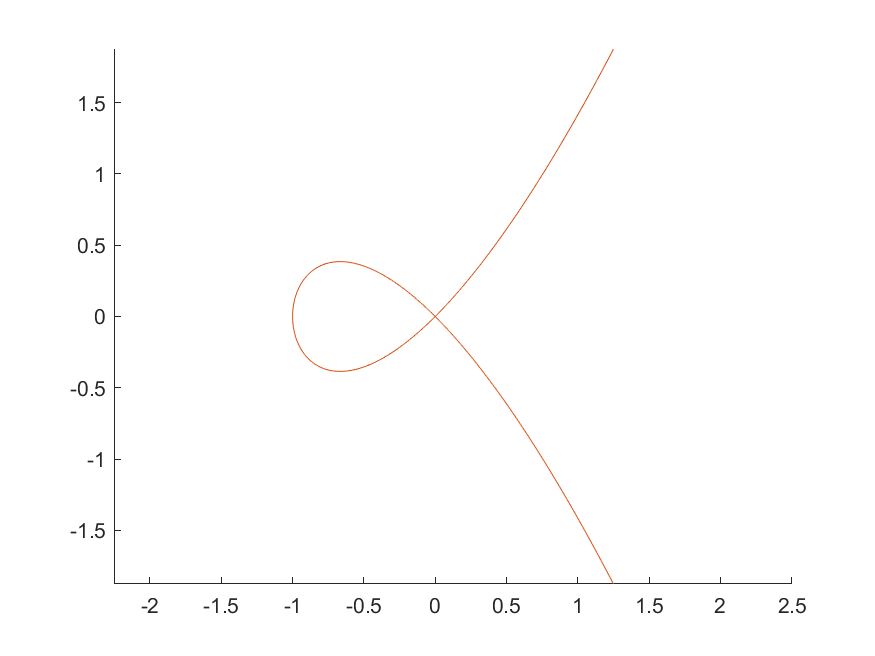
\includegraphics[width=0.7\columnwidth]{loop.png}
	\captionof{figure}{Loop}
	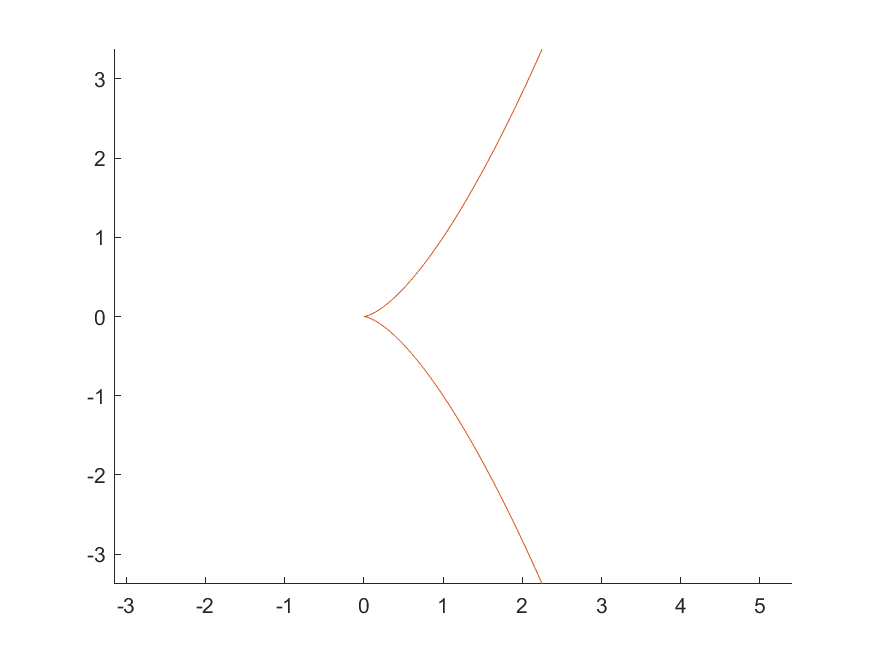
\includegraphics[width=0.7\columnwidth]{cusp.png}
	\captionof{figure}{Špica}
	\column{.5\textwidth}
	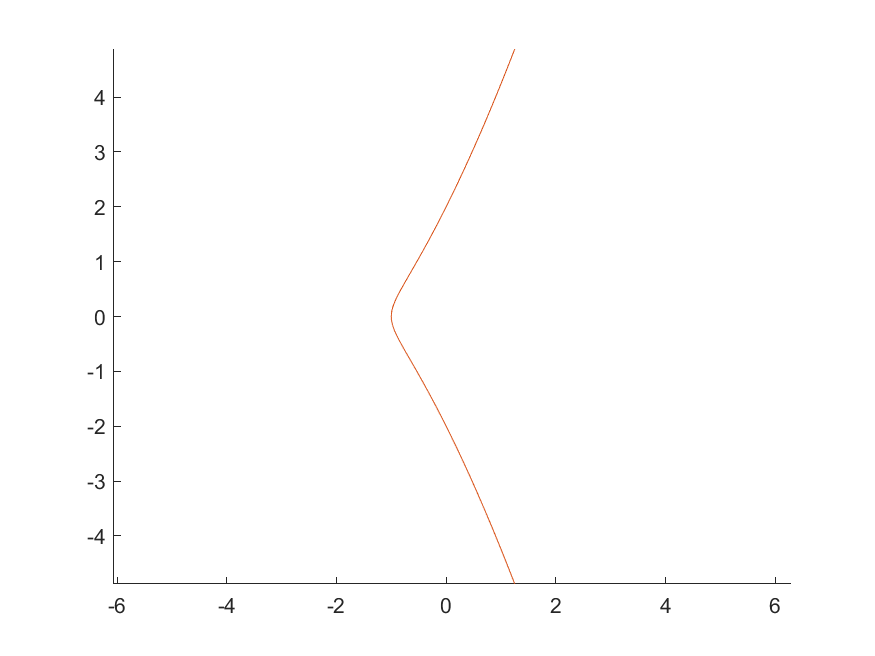
\includegraphics[width=0.7\columnwidth]{prevoj.png}
	\captionof{figure}{Dva prevoja}
	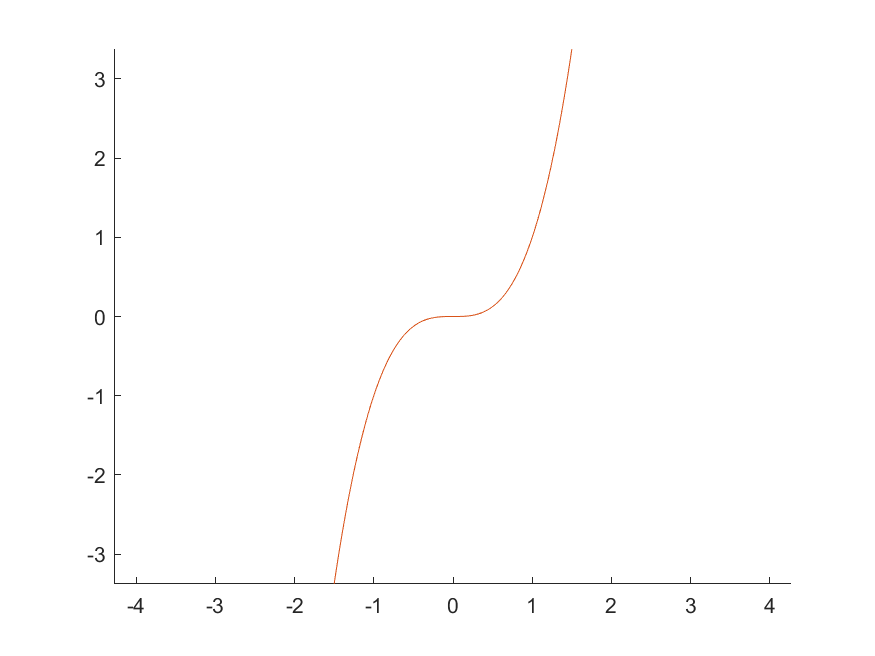
\includegraphics[width=0.7\columnwidth]{no_sing.png}
	\captionof{figure}{Brez prevojev}
\end{columns}
\end{frame}

\begin{frame} {Parametrične kubične krivulje}

Kubično parametrični krivuljo definiramo kot:
	\begin{align}
	\begin{split}
	x(t) &= a_1t^3+a_2t^2+a_3t+a_4 \\
	y(t) &= b_1t^3+b_2t^2+b_3t+b_4 \\
	&\text {za } -\infty < t < \infty \text{,}
	\label{param}
	\end{split}
	\end{align}
	njeno ukrivljenost $K$ pa:
	\[K = \frac{\frac{dx}{dt}\frac{d^2y}{dt^2} - \frac{dy}{dt}\frac{d^2x}{dt^2}}{\left((\frac{dx}{dt})^{2} +(\frac{dy}{dt})^2\right)^{3/2}}\text{.}\]

\end{frame}


\begin{frame}{Ukrivljenost}
Imenovalec iz enačbe za $K$ lahko zapišemo sledeče:
\[\frac{dx}{dt}\frac{d^2y}{dt^2} - \frac{dy}{dt}\frac{d^2x}{dt^2} = 2(At^2 + Bt +C) = 2F(t) \text{,}\]
kjer velja
	\begin{align*}
	A &= 3(a_2b_1-a_1b_2)\\
	B &= 3(a_3b_1 -a_1b_3) \\
	C &= a_3b_2-a_2b_3 \text{.}
	\end{align*}
Označimo:
\[\Delta = B^2- 4AC\]
\end{frame}

\begin{frame}{Oblike krivulj}
	\begin{trditev}
		Potreben in zadosten pogoj, da bo krivulja \eqref{param} imela špico, če je $A \neq 0$, je $\Delta = 0$.
	\end{trditev}
	\begin{trditev}
		Če krivulja \eqref{param} ni premica, bo vsebovala največ eno špico.
	\end{trditev}
	\begin{trditev}
		Potreben in zadosten pogoj, da bo krivulja \eqref{param} bo vsebovala loop (prevod??), je $\Delta <0$.
	\end{trditev}
		
\end{frame}

\begin{frame}{Krivulje na intervalu}
	V nadaljevanju bomo obravnavali lastnosti krivulj na nekem intervalu $[t_2,t_3]$. Za $t_2 \leq t \leq t_3$ lahko enačbo \eqref{param} zapišemo sledeče:
	\begin{align}
	\begin{split}
		x(t) &= a_1(t-t_2)^3+a_2(t-t_2)^2+a_3(t-t_2)+a_4 \\
		y(t) &= b_1(t-t_2)^3+b_2(t-t_2)^2+b_3(t-t_2)+b_4 
		\label{int}
	\end{split}
	\end{align}
	imenovalec v enačbi ukrivljenosti $K$ pa se izraža kot:
	 \begin{align*}
	 &\frac{dx}{dt}\frac{d^2y}{dt^2} - \frac{dy}{dt}\frac{d^2x}{dt^2} = 2(A(t-t_2)^2 + B_1(t-t_2) +_2C_1) = \\
	 &2(A(t-t_3)^2 + B_2(t-t_3) +_2C_2) = 
	 2F_1(t) \text{,}
	 \end{align*}
	 
	 kjer velja
	 	\begin{align*}
	 A &= 3(a_2b_1-a_1b_2)\\
	 B_1 &= 3(a_3b_1 -a_1b_3)  \qquad B_2 = B_1 +2A(t_3-t_2) \\
	 C_1 &= a_3b_2-a_2b_3  \qquad C_2 = C_1 +A(t_3-t_2)^2+B_1(t_3-t_2) \text{.}
	 \end{align*}
	
 \end{frame}

\begin{frame}{Klasifikacija krivulj na intervalu}
	Definiramo še $\Delta_1$ kot:
	\[  \Delta_1= B_1 - 4AC_1 \]
	\begin{trditev}
		Potrebni in zadostni pogoji, da bo krivulja \eqref{int} vsebovala loop so:
		\begin{itemize}
			\item  $\Delta_1 <0$
			\item $B^2_1 \geq 3AC_1$ in $B^2_2 \geq 3AC_2$
			\item $F'_1(t_2) F'_1(t_3) \leq 0$.
		\end{itemize}
	\end{trditev}
	\begin{trditev}
	Če je $A \neq 0$, sta naslednja pogoja potrebna in zadostna, da bo krivulja \eqref{int} vsebovala špico:
	\begin{itemize}
		\item  $\Delta_1 =0$
		\item $F'_1(t_2) F'_1(t_3) \leq 0$.
	\end{itemize}
\end{trditev}
\end{frame}

\begin{frame}{Klasifikacija krivulj na intervalu}
	\begin{trditev}
		Naslednji pogoji so potrebni in zadostni za različne vrste prevojev na krivulji \eqref{int}:
		\begin{itemize}
			\item Prevoj bo na intervalu $(t_2, t_3)$, če bo veljalo:
			$F_1(t_2)F_1(t_3) <0$.
			\item Prevoj bo pri parametru $t_2$ (oziroma $t_3$), če bo
			$\Delta_1 > 0$ in $F_1(t_2) = 0$ (oziroma $F_1(t_3) = 0$).
			\item Interval $(t_2, t_3)$ bo vseboval dva prevoja, če bo $\Delta_1 >0 $, $F_1(t_2)F'_1(t_2) <0$, $F_1(t_3)F'_1(t_3) >0$ in $F_1(t_2)F_1(t_3) >0$. 
		\end{itemize}
	\end{trditev}
	\begin{trditev}
		Potrebna in zadostna pogoja, da krivulja \eqref{int} ne bo imela prevojev, sta:
		\begin{itemize}
			\item $\Delta_1 \leq 0$ ali $F_1(t_2)F_1(t_2) > 0$
			\item $F'_1(t_2)F'_1(t_3)>0$ ali $F_1(t_2)A \leq 0$.
		\end{itemize}
	\end{trditev}
\end{frame}

\section{B-zlepki}
\begin{frame}{B-zlepki}
	
\end{frame}

\begin{frame}{Primer}
	\begin{columns}[t]
		\column{.5\textwidth}
		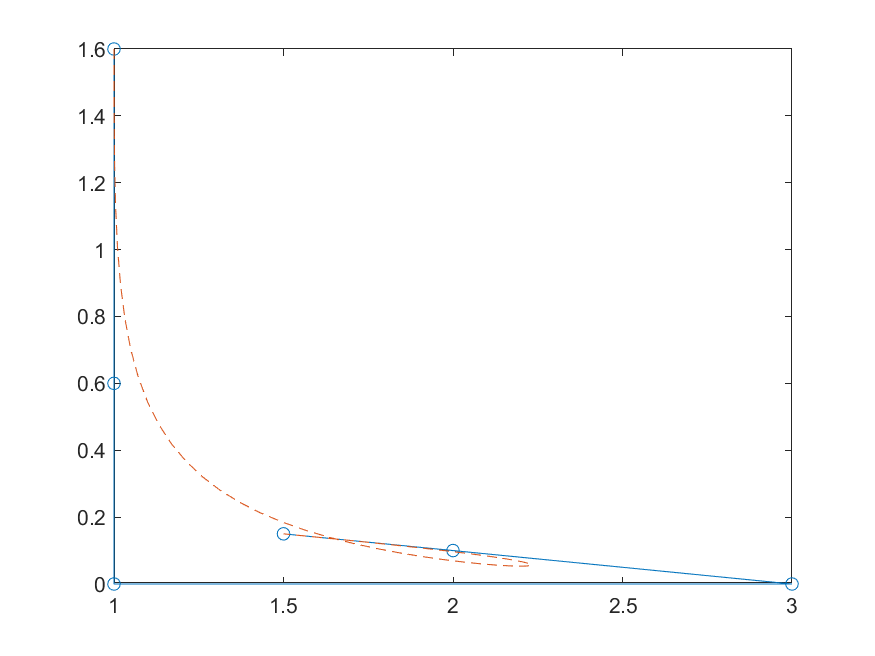
\includegraphics[width=0.7\columnwidth]{bloop.png}
		\captionof{figure}{Loop}
		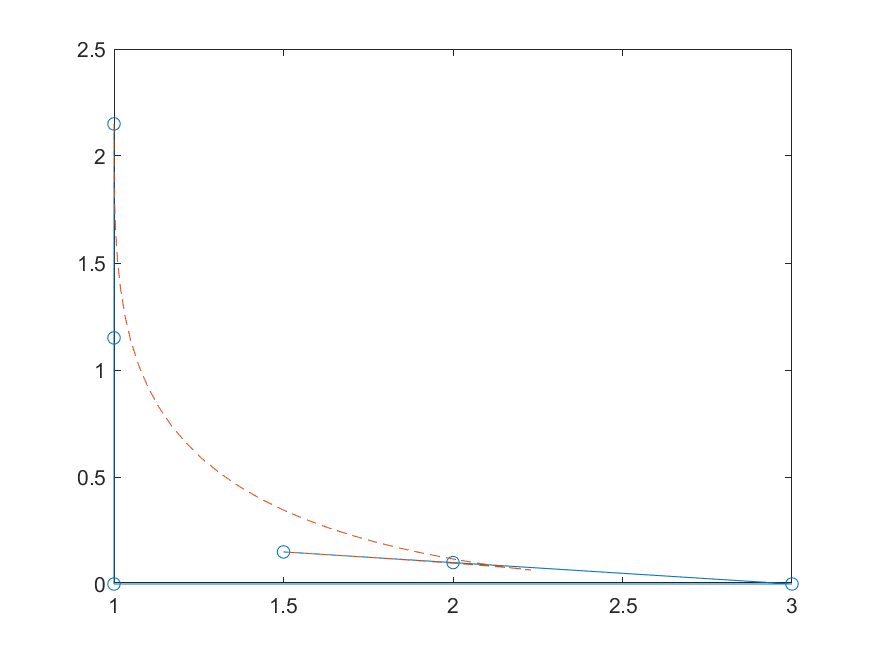
\includegraphics[width=0.7\columnwidth]{bcusp.png}
		\captionof{figure}{Špica}
		\column{.5\textwidth}
		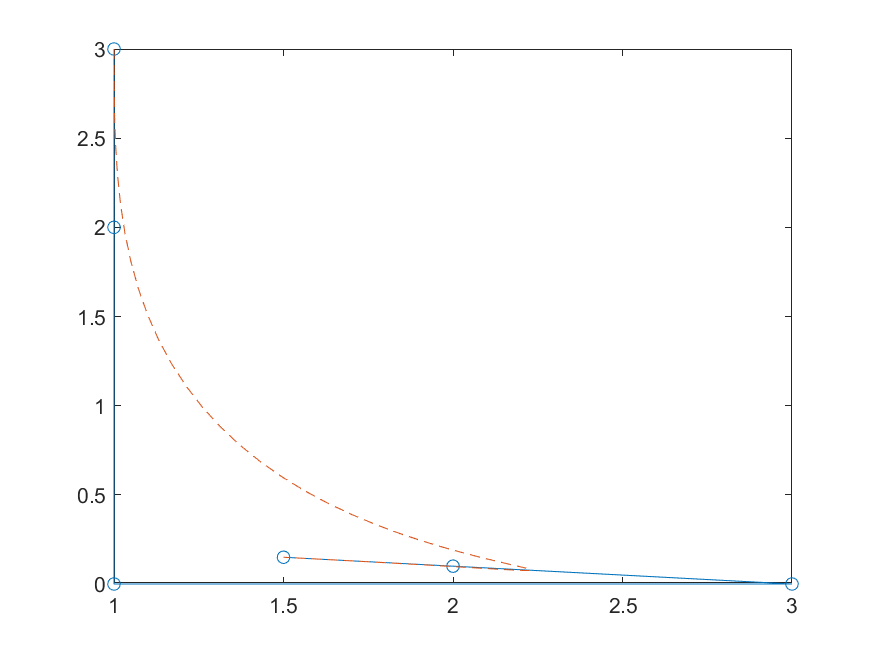
\includegraphics[width=0.7\columnwidth]{bprevoj.png}
		\captionof{figure}{Dva prevoja}
		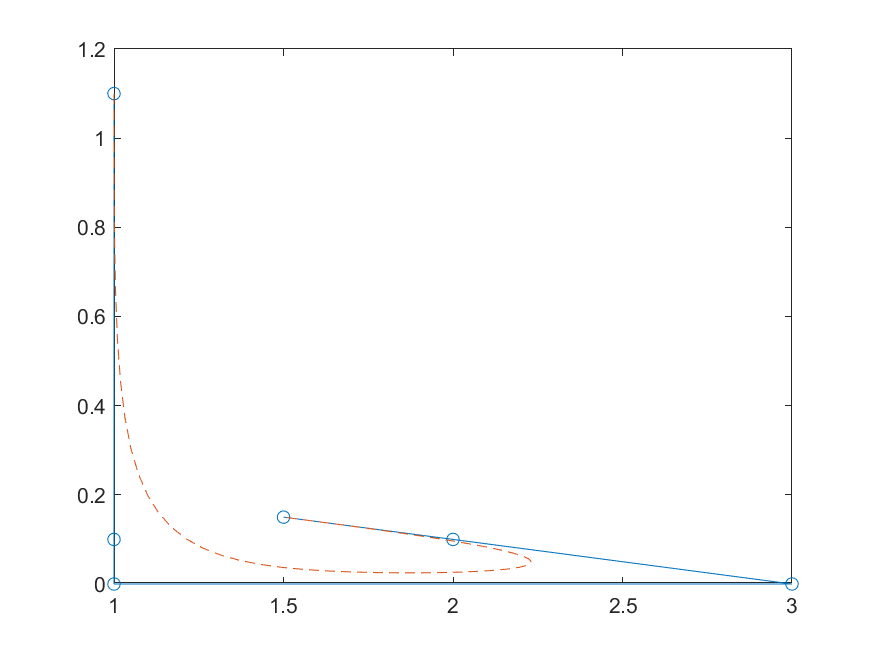
\includegraphics[width=0.7\columnwidth]{bno_sing.png}
		\captionof{figure}{Brez prevojev}
	\end{columns}
\end{frame}

\section{B-zlepki}
\begin{frame}{Uvod v B-zlepke}
	B-zlepki reda n so bazne funkcije za "spline functions" istega reda, definirane na istih vozlih. Kar pomeni, da lahko vse "spline functions" enolično predstavimo kot linearno kombinacijo B-zlepkov.
	\begin{definicija}
	Rekurzivna formula za B-zlepke:\\
	$B_{i,k}(x)= \frac{x-t_i}{t_{i+k}-t_i} B_{i,k-1}(x) +  \frac{t_{i+k+1}-x}{t_{i+k+1}-t_{i+1}} B_{i+1,k-1}(x) $

	
  $B_{i,0}(x) =
  \begin{cases}
    1 & \text{; $t_i \le x \le t_{i+1}$} \\
    0 & \text{;sicer}
  \end{cases}$

	\end{definicija}
\end{frame}

\section{}
\begin{frame}
\begin{center}
HVALA ZA POZORNOST! 
\end{center}
\end{frame}

 
\end{document}

